\documentclass[a4paper,11pt]{article}
\usepackage[utf8]{inputenc}
\usepackage[spanish]{babel}
\usepackage[affil-it]{authblk}
\usepackage{enumerate}
\usepackage{graphicx}
\usepackage{hyperref}
\usepackage{amsmath}
\usepackage{amssymb}
\usepackage{cancel}
\usepackage[usenames, dvipsnames]{color}
\usepackage{tikz}
\usepackage[labelfont=bf]{caption}
\usepackage{subcaption} %Multiple images
\usepackage{multicol} % Multiple columns
\usepackage{float}
\usepackage{cleveref}
\usepackage{relsize} % bigger math symbols
\usepackage[margin=1.1in]{geometry}
\usepackage[titletoc,toc,title]{appendix}
\usepackage{enumitem}
\usepackage{etoolbox}
\usepackage{mdframed} %frame theorems
\usetikzlibrary{calc}
\numberwithin{equation}{section}

% Footnotes with symbols

\makeatletter
\def\@fnsymbol#1{\ensuremath{\ifcase#1\or \dagger\or \ddagger\or
   \mathsection\or \mathparagraph\or \|\or **\or \dagger\dagger
   \or \ddagger\ddagger \else\@ctrerr\fi}}
\makeatother

\renewcommand{\thefootnote}{\fnsymbol{footnote}}

% Cool letters 
%Filename:      Typocaps.fd
%Created by:    MLO
%Creation date: 2003/04/02

% This file should be put in a TeX input directory

\ProvidesFile{Typocaps.fd}
   [2003/04/02 Font definition file for U/Typocaps]

\DeclareFontFamily{U}{Typocaps}{}

\DeclareFontShape{U}{Typocaps}{xl}{n}{
   <-> Typocaps
}{}

\endinput


% Footer
\usepackage{fancyhdr}
\pagestyle{fancy}
\fancyhf{}
\cfoot{\fontsize{15pt}{15pt}\usefont{U}{Typocaps}{xl}{n} 
gigantium humeris insidentes}

% Big Pictures
\usepackage[export]{adjustbox}

% Enviroment for theorems
\newmdtheoremenv[frametitle=Teorema]{theo}{Theorem}

% Circled words
\newcommand{\circled}[2][]{%
  \tikz[baseline=(char.base)]{%
    \node[shape = circle, draw, inner sep = 1pt]
    (char) {\phantom{\ifblank{#1}{#2}{#1}}};%
    \node at (char.center) {\makebox[0pt][c]{#2}};}}
\robustify{\circled}

%Appendices in spanish
\renewcommand{\appendixname}{Ap\'endices}
\renewcommand{\appendixtocname}{Ap\'endices}
\renewcommand{\appendixpagename}{Ap\'endices}

%Zero delimiter
\newcommand{\zerodel}{.\kern-\nulldelimiterspace}

%Columns separation
\setlength{\columnsep}{1cm}

%Indentation
\setlength{\parindent}{0ex}

%Multiple References

\crefrangelabelformat{equation}{(#3#1#4--#5\crefstripprefix{#1}{#2}#6)}

\usepackage{xparse}

%Boxes

\newcommand*{\boxcolor}{blue}
\makeatletter
\renewcommand{\boxed}[1]{\textcolor{\boxcolor}{%
\tikz[baseline={([yshift=-1ex]current bounding box.center)}] \node [rectangle, minimum width=1ex,rounded corners,draw] {\normalcolor\m@th$\displaystyle#1$};}}
 \makeatother

%Constantes
\newcommand{\euler}{\mathrm{e}}
\newcommand{\im}{i}

%Lemas, teoremas, definiciones y pruebas
\newcommand{\definicion}{\textbf{Definición: }}
\newcommand{\lema}{\textbf{Lema: }}
\newcommand{\teorema}{\textbf{Teorema: }}
\newcommand{\prueba}{\textbf{Prueba: }}
\newcommand{\proposicion}{\textbf{Proposición: }}
\newcommand{\corolario}{\textbf{Corolario: }}

% Definición de las secciones y su numeración

\makeatletter
\def\@seccntformat#1{%
  \expandafter\ifx\csname c@#1\endcsname\c@section\else
  \csname the#1\endcsname\quad
  \fi}
\makeatother

\begin{document}

\begin{titlepage}
\thispagestyle{fancy}

\newcommand{\HRule}{\rule{\linewidth}{0.5mm}} % Defines a new command for the horizontal lines, change thickness here

\center % Center everything on the page
 
%----------------------------------------------------------------------------------------
%	HEADING SECTIONS
%----------------------------------------------------------------------------------------

\textsc{\LARGE Universidad Nacional Autónoma de México}\\[0.3cm] % Name of your university/college

%----------------------------------------------------------------------------------------
%	LOGO SECTION
%----------------------------------------------------------------------------------------


\includegraphics[scale=0.17]{unam}

%----------------------------------------------------------------------------------------
%	SUBHEADING SECTIONS
%----------------------------------------------------------------------------------------

\textsc{\Large Electrodinámica Clásica}\\[0.5cm] % Major heading such as course name
\textsc{\large Semestre 2016-II}\\[0.5cm] % Minor heading such as course title

%----------------------------------------------------------------------------------------
%	TITLE SECTION
%----------------------------------------------------------------------------------------

\HRule \\[0.4cm]
{ \huge \bfseries Tarea \# 3. Campos Multipolares.}\\[0.2cm] % Title of your document
\HRule \\[1cm]
 
%----------------------------------------------------------------------------------------
%	AUTHOR SECTION
%----------------------------------------------------------------------------------------
\setcounter{footnote}{0}
\center
\large
\emph{Autor:} \\ % Your name
\Large Favio \textsc{Vázquez}\footnote[1]{\href{mailto:favio.vazquez@correo.nucleares.unam.mx}{favio.vazquez@correo.nucleares.unam.mx}}

%----------------------------------------------------------------------------------------
%	COOL IMAGE SECTION
%----------------------------------------------------------------------------------------

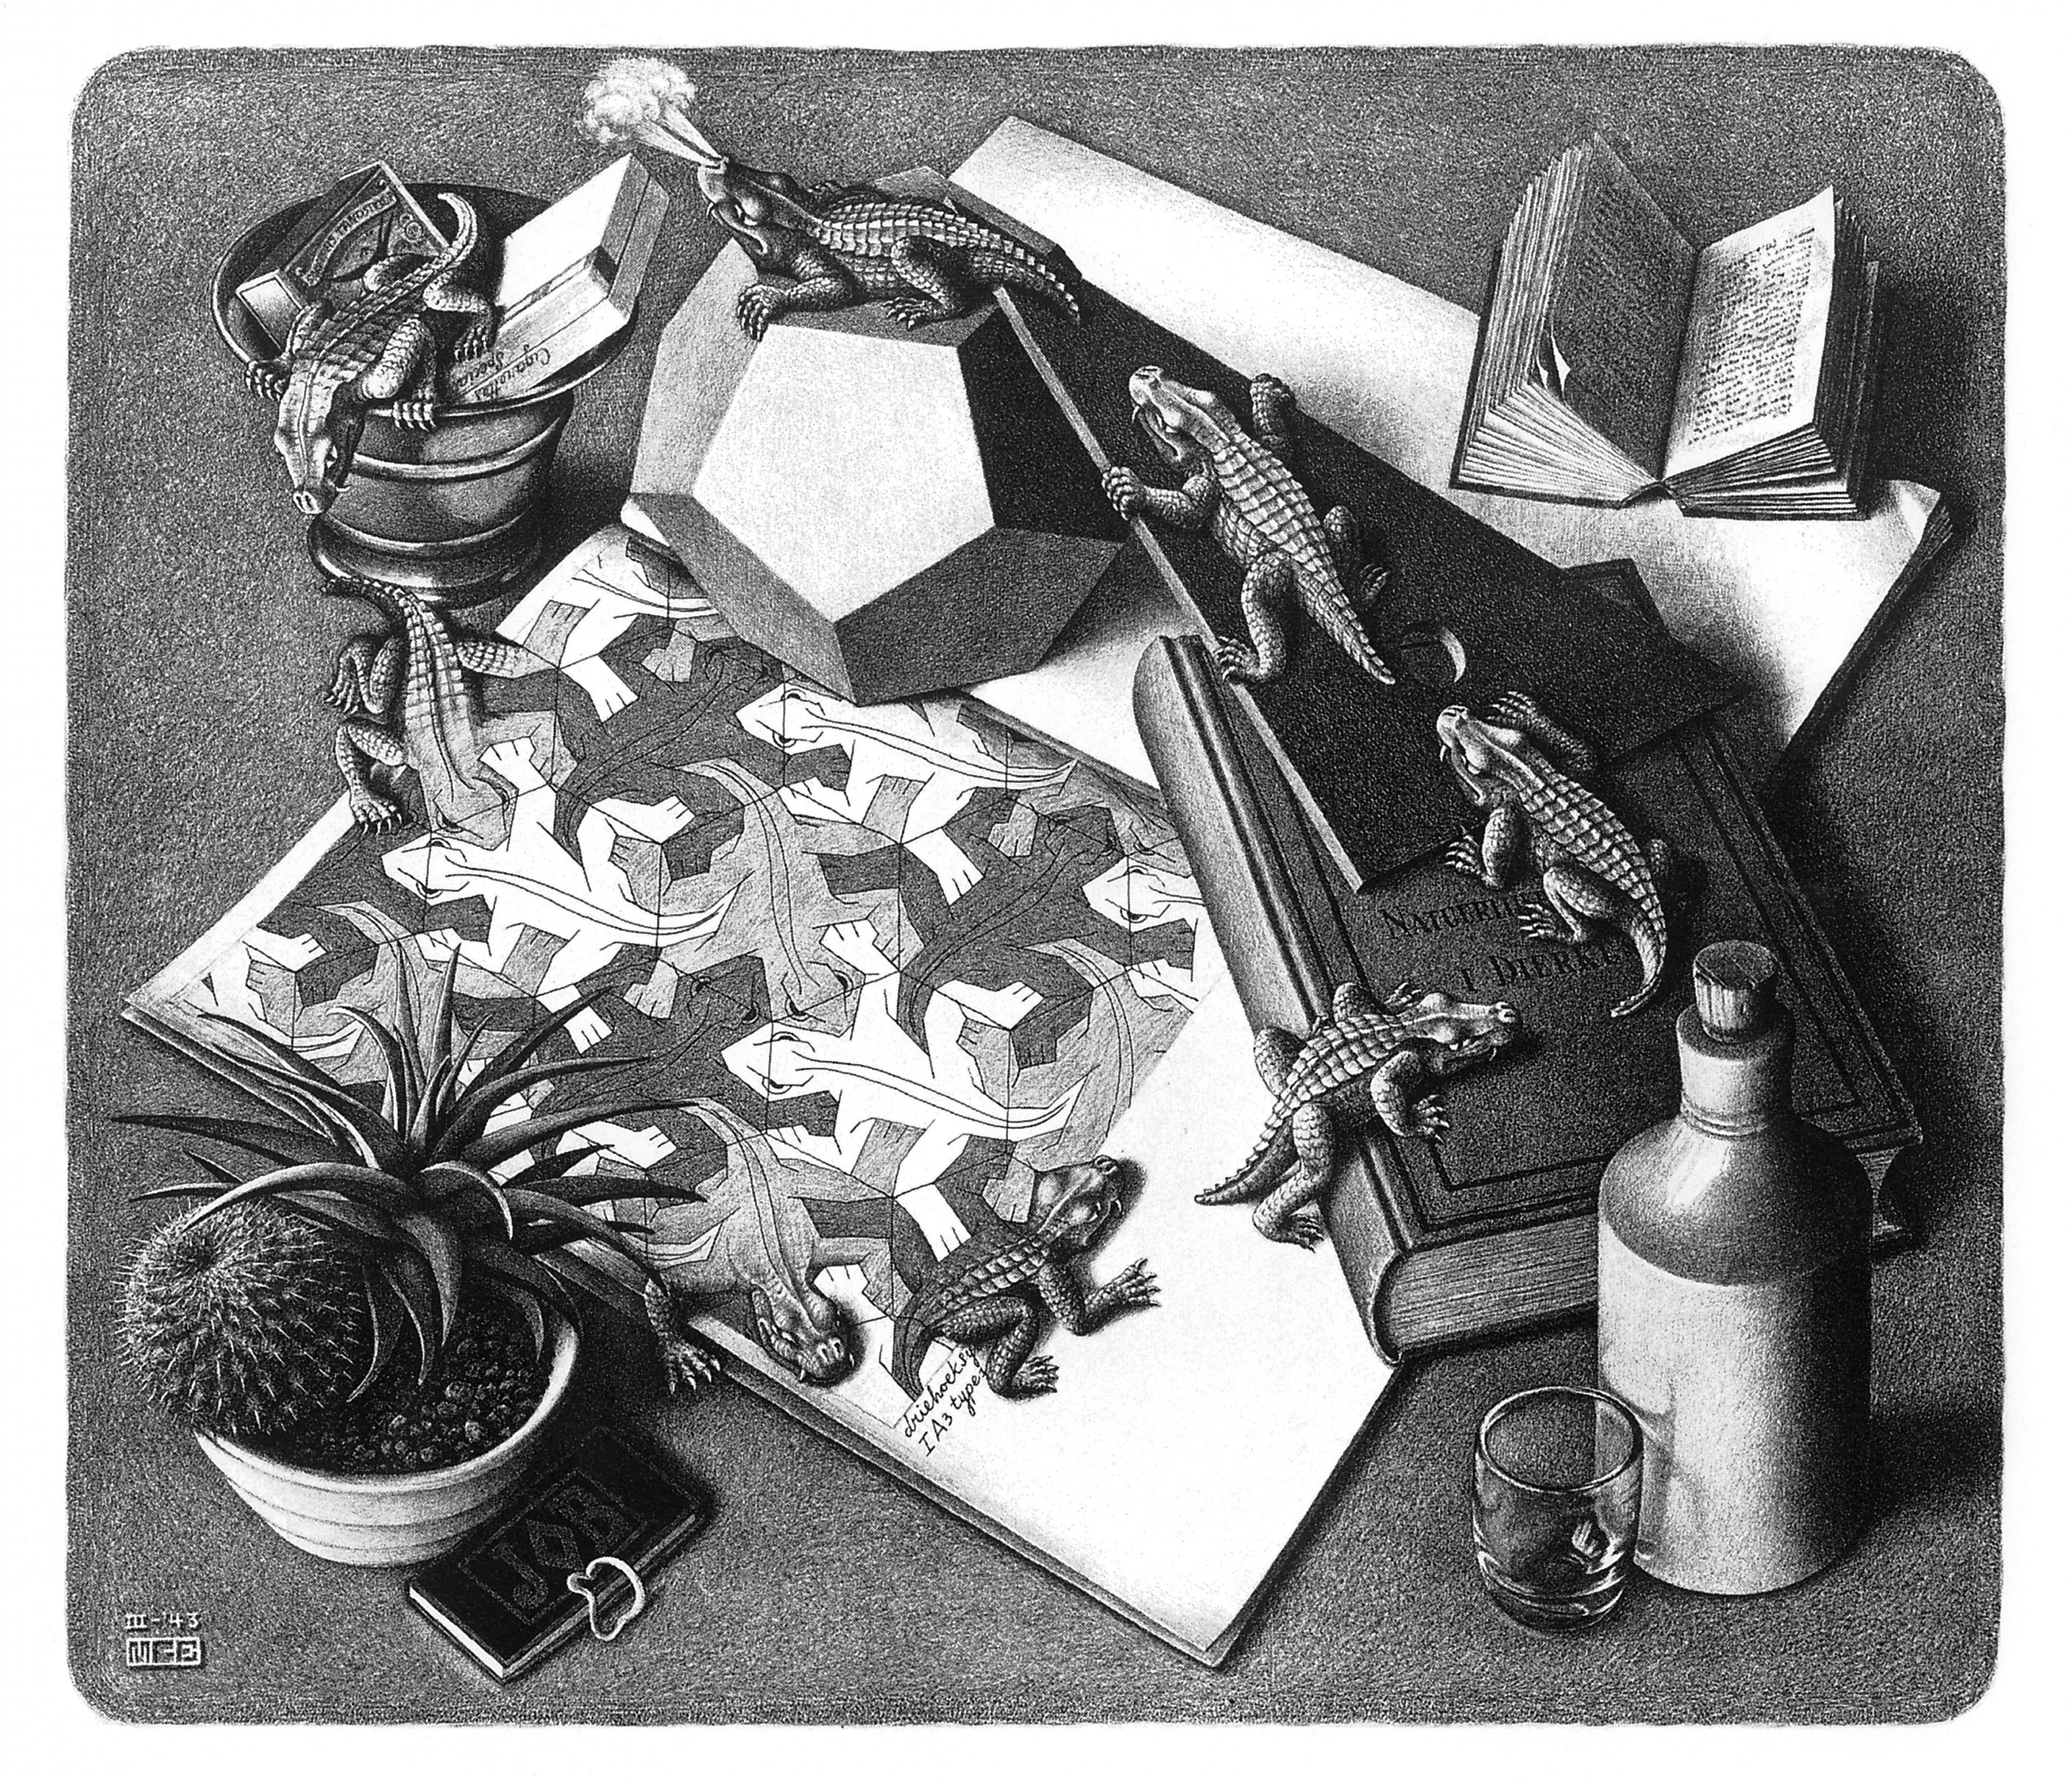
\includegraphics[scale=0.135]{reptilesEscher}

%----------------------------------------------------------------------------------------

\vfill % Fill the rest of the page with whitespace

\end{titlepage}

% ---------------------------------------------------------------------------------------
%         HEADER
%----------------------------------------------------------------------------------------

\fancyhead[L]{Favio Vázquez}
\fancyhead[R]{\thepage}

%----------------------------------------------------------------------------------------
\setcounter{footnote}{0}
\renewcommand*{\thefootnote}{\arabic{footnote}}

\section{Problema 1. Problema 2.1 de Classical Electromagnetic Radiation
de Marion y Heald \cite{marion2}.}

Muestre que el campo eléctrico en el eje polar de un dipolo $\mathbf{p}$ es 
$2\mathbf{p}/z^3$, mientras que en el plano ecuatorial es $-\mathbf{p}/r^3$. Use 
este argumento elemental para mostrar, resolviendo el dipolo en dos componentes, que 
el campo en un punto arbitrario es 

$$
E(r,\theta) = \frac{p(2\cos{\theta}\mathbf{e_r} + \sen{\theta}\mathbf{e_\theta})}{r^3}
$$

\vspace{.3cm}

\underline{Solución:} \vspace{.3cm}

Para calcular el campo eléctrico en el eje polar proponemos la siguiente geometría,

\begin{figure}[H]
 \center 
 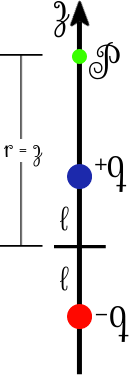
\includegraphics[scale=0.5]{problema1fig1}
 \caption{Campo eléctrico de un dipolo en el eje polar.}
 \label{fig:problema1fig1}
\end{figure}

y mediremos el campo en un punto $P$ a una distancia $z$ del origen. El potencial 
eléctrico en el punto $P$ debido a las cargas $q$ y $-q$ será 

\begin{equation}
 \Phi = \frac{q}{r_{+q}} - \frac{q}{r_{-q}},
\end{equation}

\begin{equation}
 \Phi = \frac{q}{(z + l)} - \frac{q}{(z - l)},
\end{equation}

y utilizando el hecho de que\footnote{ep = eje polar.} 

\begin{equation}
 E_{ep} = - \text{grad} \, \Phi,
\end{equation}

vemos que 

\begin{equation}
 E_{ep} = \frac{q}{(z - l)^2} - \frac{q}{(z + l)^2}.
\end{equation}

Que podemos escribir como 

\begin{equation}
 E_{ep} = \frac{q}{z^2}\left[\frac{1}{\left(1 - \frac{l}{z}\right)^2} - 
 \frac{1}{\left(1 + \frac{l}{z}\right)^2}\right],
\end{equation}

y asumiendo que $z \gg l$ podemos expandir en series de Maclaurin obteniendo 

\begin{equation}
 E_{ep} = \frac{q}{z^2}\left[\left(1 + \frac{2l}{z} + \dots \right) - 
 \left(1 - \frac{2l}{z} + \dots \right) \right]
\end{equation}

\begin{equation}
 E_{ep} = \cancel{\frac{q}{z^2}} + \frac{q2l}{z^3} - \cancel{\frac{q}{z^2}} +
 \frac{q2l}{z^3},
\end{equation}

\begin{equation}
 \therefore E_{ep} = \frac{4ql}{z^3},
\end{equation}

y ahora recordando que $p = 2ql$, y que $\mathbf{E}$ es paralelo a $\mathbf{p}$, 
encontramos que 

\begin{equation}
 \boxed{\mathbf{E}_{ep} = \frac{2\mathbf{p}}{z^3}}.
\end{equation}

\hspace{10cm}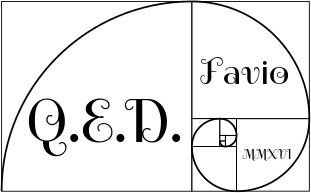
\includegraphics[scale=0.25]{logoQED}

\vspace{.2cm}

Ahora para el plano ecuatorial proponemos la siguiente geometría, 

\begin{figure}[H]
 \center 
 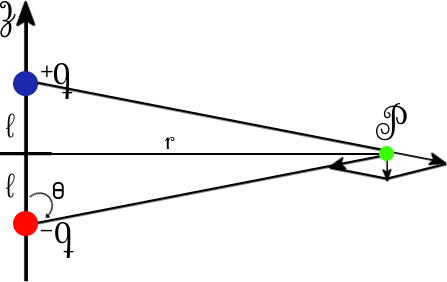
\includegraphics[scale=0.5]{problema1fig2}
 \caption{Campo eléctrico de un dipolo en el plano ecuatorial.}
 \label{fig:problema1fig2}
\end{figure}

En este caso el campo eléctrico en el punto $P$ a una distancia $r$ del origen, 
ubicado en el plano ecuatorial podemos escribirlo como\footnote{pe = plano ecuatorial.}

\begin{equation}
 E_{pe} = \frac{q}{(r^2+a^2)} + \frac{q}{(r^2+a^2)} = 2 \frac{q}{(r^2+a^2)},
\end{equation}

ahora el campo resultante $E$ en la dirección vertical se cancela por la simetría 
del problema, manteniéndose solo la parte horizontal, es decir (ver figura
\eqref{fig:problema1fig2})

\begin{equation}
 E_{pe} = \frac{2q}{(r^2+a^2)}\cos{\theta},
\end{equation}

y viendo la figura \eqref{fig:problema1fig2} vemos que podemos escribir 

\begin{equation}
 \cos{\theta} = \frac{\text{CA}}{\text{HIP}} = \frac{l}{(r^2+a^2)^2},
\end{equation}

entonces 

\begin{equation}
 E_{pe} = \frac{2q}{(r^2+a^2)} \frac{l}{(r^2+a^2)^2} = \frac{2ql}{(r^2+a^2)^{3/2}},
\end{equation}

que podemos escribir como 

\begin{equation}
 E_{pe} = \frac{2ql}{r^3}\left(1 + \frac{l^2}{r^2} \right),
\end{equation}

y en el límite cuando $r \gg l \rightarrow l^2/r^2 \approx 0$,

\begin{equation}
 \therefore E_{pe} = \frac{2ql}{r^3},
\end{equation}

y recordando que $p = 2ql$ y que el momento dipolar va en sentido de la $-z$, que 
es el sentido opuesto del campo eléctrico (ver figura \eqref{fig:problema1fig2}) nos queda 

\begin{equation}
 \boxed{\mathbf{E}_{pe} = - \frac{\mathbf{p}}{r^3}}.
 \label{eq:campoElecDipoloEcuador}
\end{equation}

\hspace{10cm}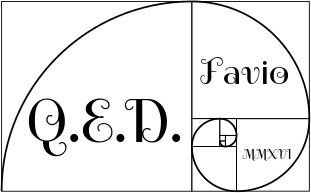
\includegraphics[scale=0.25]{logoQED}

\vspace{.2cm}

Ahora usando estos resultados podemos demostrar la ecuación solicitada. El campo 
eléctrico en un punto $P$ arbitrario será la superposición del campo en el eje polar 
de la componente $p_{\parallel} = p \cos{\theta}$, y el campo en el plano ecuatorial de la 
componente $p_{\bot} = p\sen{\theta}$, esto se puede ver en la figura 
\eqref{fig:problema1fig3}.

\begin{figure}[H]
 \center 
 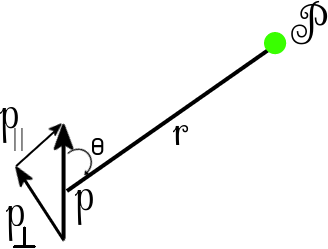
\includegraphics[scale=0.5]{problema1fig3}
 \caption{Campo eléctrico de un dipolo en un punto arbitrario del espacio.}
 \label{fig:problema1fig3}
\end{figure}

\begin{equation}
 \mathbf{E}(r,\theta) = \frac{2p_\parallel}{r^3} \mathbf{e}_r + 
 \frac{p_\bot}{r^3}\mathbf{e}_\theta,
\end{equation}

donde el signo negativo del campo en el plano ecuatorial se cancela por el hecho de 
que, genéricamente, $\mathbf{e}_\theta$ va en el sentido opuesto de $\mathbf{p}$, 
entonces utilizando la figura \eqref{fig:problema1fig3} vemos que 

\begin{equation}
 \boxed{\mathbf{E}(r,\theta) = \frac{p}{r^3}(2\cos{\theta}\mathbf{e}_r + 
 \sen{\theta}\mathbf{e}_\theta)}.
\end{equation}

\hspace{10cm}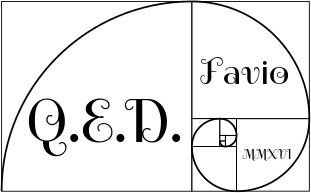
\includegraphics[scale=0.25]{logoQED}

\section{Problema 2. Problema 2.2 de Classical Electromagnetic Radiation
de Marion y Heald \cite{marion2}.}

El campo magnético de la Tierra es aproximadamente el de un dipolo. Calcule el momento 
dipolar magnético usando el hecho de que la componente horizontal del campo de la 
Tierra en su superficie es aproximadamente $0.23$ G a una latitud magnética de 
$40^\circ$.

\vspace{.3cm}

\underline{Solución:} \vspace{.3cm}

Ya que podemos aproximar el campo magnético de la Tierra como un dipolo, y la geometría
de los campos externos de un dipolo eléctrico y magnético es la misma, podemos utilizar 
las ecuaciones que obtuvimos en el anterior problema, solamente reemplazando $\mathbf{p}$ 
por $\mathbf{m}$ y $\mathbf{E}$ por $\mathbf{B}$. La componente horizontal, asumiendo 
una Tierra perfectamente esférica, es simplemente la componente $\mathbf{e}_\theta$; 
y recordando que el ángulo de latitud $\theta_l$ se mide desde el ecuador, podemos 
escribir\footnote{Ver ecuación \eqref{eq:campoElecDipoloEcuador}.}

\begin{equation}
 B_{\text{horizontal}} = \frac{m\cos{\theta_l}}{R_t^3},
 \label{eq:campoMagnDipoloTierra}
\end{equation}

  donde $R_t$ es el radio de la tierra y  $\theta_l$ se mide de acuerdo a la siguiente 
figura 


\begin{figure}[H]
 \center 
 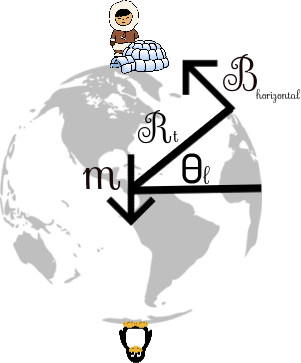
\includegraphics[scale=0.5]{problema2fig1}
 \caption{Campo magnético de la tierra. El dipolo magnético apunta 
 hacia la Antártica con los pingüinos.}
 \label{fig:problema2fig1}
\end{figure}

Debido a que el radio de la tierra es aproximadamente $R_t = 6.37 \times 10^8$ cm, 
resolviendo \eqref{eq:campoMagnDipoloTierra} para $m$ nos queda, 

\begin{equation}
 \boxed{m = \frac{(0.23 \text{ G})(6.37 \times 10^8 \text{ cm})^3}{\cos{40^\circ}} = 
 7.8 \times 10^{25} \text{ G}\text{ cm}^3}.
\end{equation}

El dipolo magnético de la tierra apunta hacia la Antártica y por lo tanto las líneas 
del campo magnético retornan hacia el Ártico (con los esquimales) en el norte de la 
superficie de la Tierra.

\section{Problema 3. Problema 2.3 de Classical Electromagnetic Radiation
de Marion y Heald \cite{marion2}.}

Muestre que el momento dipolar eléctrico de un sistema de cargas es independiente 
de la elección del origen si el sistema tiene carga neta igual a cero.

\vspace{.3cm}

\underline{Solución:} \vspace{.3cm}

Podemos imaginarnos la geometría del sistema colocando una colección de cargas 
$q_\alpha$ a una distancia $r'_\alpha$ del origen original $O$, y a una distancia 
$R'_\alpha = r'_\alpha - r_O$ del otro origen que llamamos $O'$, y donde $r_O$ es 
la distancia entre los dos orígenes, representada en la siguiente figura 

\begin{figure}[H]
 \center 
 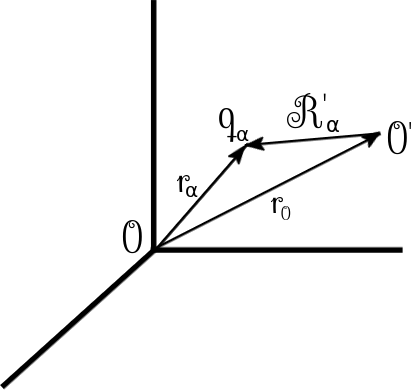
\includegraphics[scale=0.5]{problema3fig1}
 \caption{Geometría de una colección de cargas $q_\alpha$ con respecto a dos 
 orígenes diferentes.}
 \label{fig:problema3fig1}
\end{figure}

Según la ecuación (2.22) de Marion y Heald \cite{marion2}, el momento dipolar del sistema 
de cargas es 

\begin{equation}
 \mathbf{p} = \sum_\alpha q_\alpha r'_\alpha,
\end{equation}

y si expresamos los vectores de posición en términos del origen $O'$, tenemos 

\begin{equation}
 r'_\alpha = r_O + R'_\alpha,
\end{equation}

y luego 

\begin{equation}
 \mathbf{p} = \sum_\alpha = q_\alpha(r_O + R'_\alpha) = r_O \sum_\alpha q_\alpha + 
 \sum_\alpha q_\alpha R'_\alpha,
\end{equation}

pero si el sistema tiene carga neta igual a cero entonces $\sum_\alpha q_\alpha = 0$, y 
el primer término de la ecuación anterior se hace cero, y por lo tanto el momento 
dipolar es independiente de la posición de $r_O$ del origen. Podemos decir 
entonces que el momento dipolar de un sistema de cargas es independiente de la elección
del origen del sistema, siempre y cuando el sistema tenga una carga neta igual a 
cero.

\hspace{10cm}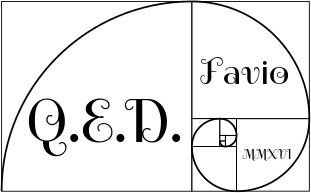
\includegraphics[scale=0.25]{logoQED}

\section{Problema 4. Problema 2.3 de Classical Electromagnetic Radiation
de Marion y Heald \cite{marion2}.}

Muestre que la fuerza en un dipolo eléctrico es $\mathbf{F} = (\mathbf{p}\cdot 
\mathbf{grad})\mathbf{E}$. Luego considere la interacción de una carga $q$ y un dipolo 
$\mathbf{p}$ que están a una distancia $r$, con el dipolo orientado perpendicular a 
la línea que los une. Calcule la fuerza (vectorial)

\begin{enumerate}[label=\textbf{(\alph*)}]
\item en q debido a $\mathbf{p}$, 
\item en $\mathbf{p}$ debido a q.
\end{enumerate}

Si tus resultados violan la tercera ley de Newton, inténtalo de nuevo.

\vspace{.3cm}

\underline{Solución:} \vspace{.3cm}

Si colocamos el origen de nuestro sistema (cartesiano) en el centro del dipolo, y 
expandimos el campo eléctrico en una serie de Maclaurin sobre este origen obtenemos:

\begin{equation}
 E(x,y,z) = E_0 + \left(\frac{\partial E}{\partial x} \right)_0 x + 
  \left(\frac{\partial E}{\partial y} \right)_0 y + 
   \left(\frac{\partial E}{\partial z} \right)_0 z + \dots
\end{equation}

Que en notación de Marion y Heald \cite{marion2} escribimos como 

\begin{equation}
 E(x,y,z) = E_0 + (\mathbf{r}\cdot \text{\textbf{grad}})\mathbf{E} + \dots 
\end{equation}

Ahora recordando que que $\mathbf{F} = q\mathbf{E}$ podemos sumar las fuerzas 
vectoriales de nuestro modelo de dipolo que consisten en dos cargas $\pm q$ en 
las posiciones $\pm l$ respectivamente, para obtener 

\begin{equation}
 \mathbf{F} = q[E_0 + (\mathbf{l}\cdot \text{\textbf{grad}})\mathbf{E} + \dots ]
 - q[E_0 + (\mathbf{l}\cdot \text{\textbf{grad}})\mathbf{E} + \dots ],
\end{equation}

\begin{equation}
 \therefore \mathbf{F} = 2q (\mathbf{l}\cdot \text{\textbf{grad}})\mathbf{E},
\end{equation}

y recordando la definición de momento dipolar nos queda 

\begin{equation}
 \boxed{\mathbf{F} = (\mathbf{p}\cdot \text{\textbf{grad}})\mathbf{E}}.
\end{equation}

\hspace{10cm}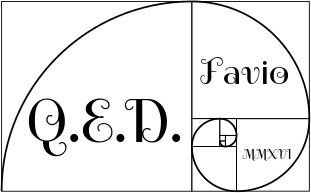
\includegraphics[scale=0.25]{logoQED}

Consideremos la interacción de una carga $q$ y un dipolo 
$\mathbf{p}$ que están a una distancia $r$, con el dipolo orientado perpendicular a 
la línea que los une. Para el caso (a), para calcular la fuerza en $q$ debido a 
$\mathbf{p}$, colocando la carga $q$ en el plano ecuatorial del dipolo, del problema 
1 sabemos que la fuerza que sentirá la partícula será\footnote{Ver ecuación 
\eqref{eq:campoElecDipoloEcuador}}

\begin{equation}
 \boxed{\mathbf{F}_{\text{p sobre q}} = q E_{pe} = - \frac{qp}{r^3}\mathbf{e}_p},
 \label{eq:dipoloPsobreQ}
\end{equation}

donde $\mathbf{e}_p$ es el vector unitario en la dirección de $\mathbf{p}$. En 
el caso (b), para calcular la fuerza en $\mathbf{p}$ debido a $q$, utilizamos 
la ecuación que derivamos al principio del problema, 

\begin{equation}
 \mathbf{F}_{\text{q sobre p}} = (\mathbf{p}\cdot \text{\textbf{grad}})\mathbf{E}(q).
\end{equation}

Ahora, el operador $(\mathbf{p}\cdot \text{\textbf{grad}})$ es el operador de 
derivada espacial en la dirección de $\mathbf{e}_p$, y podría parecer que el campo 
debido a $q$ en $p$ solo cambiaría en la dirección radial desde $q$ y por lo tanto 
la derivada en la dirección de $\mathbf{e}_p$ es cero, lo cual violaría la tercera 
ley de Newton, ya que las fuerzas que esperamos deberían ser iguales y opuestas en 
$q$ y $\mathbf{p}$; pero haciendo un estudio más detallado nos damos cuenta que 
el campo cambia de dirección, así no cambie de signo, por lo tanto la fuerza 
sobre $p$ no sería cero. Nos faltaría demostrar que en efecto es igual y opuesta 
a la fuerza sobre $q$, para esto calculamos las componentes del campo eléctrico 
en un sistema de coordenadas con origen en $q$, el eje $x$ hacia $p$ y el eje 
$y$ paralelo a $\mathbf{p}$, por lo tanto escribimos (para el campo cercano a p)

\begin{align*}
 E_x = \frac{q}{(x^2+y^2)}\frac{x}{(x^2+y^2)^{1/2}} \approx \frac{q}{x^2} \\
 E_y = \frac{q}{(x^2+y^2)}\frac{y}{(x^2+y^2)^{1/2}} \approx \frac{qy}{x^3} \\
 E_x = \frac{q}{(x^2+y^2)}\frac{z}{(x^2+y^2)^{1/2}} \approx \frac{qz}{x^3},
\end{align*}

y debido a la geometría que propusimos para el sistema el operador relevante 
será solo el correspondiente a $y$, por lo tanto reescribimos la fuerza en 
$\mathbf{p}$ debido a $q$ como 

\begin{equation}
 \mathbf{F}_{\text{q sobre p}} = p\frac{\partial}{\partial y}\left( \frac{q}{x^2} 
 \mathbf{e}_x + \frac{qy}{x^3}\mathbf{e}_y + \frac{qz}{x^3}\mathbf{e}_z\right),
\end{equation}
 
\begin{equation}
 \boxed{\therefore  \mathbf{F}_{\text{q sobre p}} = \frac{qp}{x^3}\mathbf{e}_y},
\end{equation}

que colocando $x \rightarrow r$ y $\mathbf{e}_y \rightarrow \mathbf{e}_p$ es igual y 
opuesta a \eqref{eq:dipoloPsobreQ}, de acuerdo a la tercera ley de Newton.

\section{Problema 5. Problema 2.5 de Classical Electromagnetic Radiation
de Marion y Heald \cite{marion2}.}

Muestra que un dipolo finito simple (cargas $\pm q$ localizadas en $z = \pm l/2$) 
tiene un momento cuadrupolar cero con respecto a su centro como origen.

\vspace{.3cm}

\underline{Solución:} \vspace{.3cm}

\section{Problema 6. Problema 2.6 de Classical Electromagnetic Radiation
de Marion y Heald \cite{marion2}.}

Una carga $q_1 = + 2e$ está localizada en el origen y una carga $q_2 = - e$ está 
localizada en el punto $(x,y) = (1,0)$. Calcule el potencial en los puntos $(0,5)$
y $(5,0)$ en las siguientes maneras:

\begin{enumerate}[label=\textbf{(\alph*)}]
\item Mediante un cálculo directo de $q/R$ para cada carga,
\item Considerando un término de una expansión multipolar:
\subitem - De dos términos,
\subitem - De tres términos.
\end{enumerate}

Discute la diferencia en las tasas de convergencia hacia los valores exactos para 
los dos diferentes puntos del campo.

\vspace{.3cm}

\underline{Solución:} \vspace{.3cm}

\section{Problema 7. Problema 2.7 de Classical Electromagnetic Radiation
de Marion y Heald \cite{marion2}.}

Computa el tensor cuadrupolar para la siguiente distribución de cargas:

\begin{figure}[H]
\center
 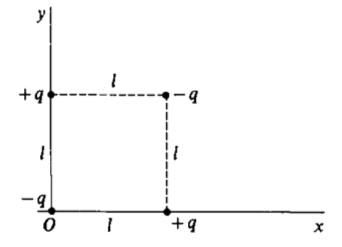
\includegraphics[scale=0.6]{problema7fig1}
\end{figure}

Diagonaliza el tensor mediante una rotación de coordenadas y encuentra el momento
cuadrupolar.

\vspace{.3cm}

\underline{Solución:} \vspace{.3cm}

\section{Problema 8. Problema 2.12 de Classical Electromagnetic Radiation
de Marion y Heald \cite{marion2}.}

La densidad de carga lineal de un anillo de radio $a$ está dada por 

$$
\lambda = \frac{q}{a}(\cos{\phi} - \sen{2\phi})
$$

\begin{enumerate}[label=\textbf{(\alph*)}]
\item Encontrar el momento monopolar, dipolar y cuadrupolar del sistema.
\item Calcular el potencial en un punto arbitrario del espacio, preciso hasta 
términos en $q/r^3$.
\end{enumerate}

\vspace{.3cm}

\underline{Solución:} \vspace{.3cm}

\begin{thebibliography}{10}
\bibitem{marion2}
J. Marion, M. Heald, \emph{Classical Electromagnetic Radiation}, 2da edición, Academic 
Press, 1965.
\end{thebibliography}

\end{document}